\documentclass[11pt,a4paper,openany]{book}

%\usepackage[german]{babel}	%in case you want to write a german thesis

%settings for generation of titlepage, index and table of content
\include{sections/Settings}

%definitions for easier costumization
\def \subtitle {Autonomous universal Mapping and Navigation}
\def \year {2021/22}
\def \authors { 
	\vspace{3mm}
	\parseauthor{System Design, Sensory Inputs, Mapping}{Lukas Leskovar}{5BHIF}\\
	\vspace{3mm}
	\parseauthor{Motion Planning, Exploration, Collision Detection}{Fabian Kleinrad}{5BHIF}}
\def \supervisor {MMag. Dr. Michael Stifter}
\def \declauthors{ Lukas Leskovar & Fabian Kleinrad}	% for two authors
% \def \declauthors{ Vor- und NACHNAME & Vor- und NACHNAME \\ Vor- und NACHNAME}	% for three authors

\addbibresource{main.bib}

\begin{document}
	\pagenumbering{none}
	
	%include titlepage
	\input{sections/titlepage}
	
	%include acknowledgements, abstract and documentation
	
	\pagestyle{plain}
	
%	\frontmatter
	
	\pagenumbering{roman}
	\input{sections/declarationof}
	
	\tableofcontents
	
	\chapter{Acknowledgement}

First and foremost, the authors would like to thank F-WuTS and robo4you for providing the equipment and facilities used during the development of the Autumn project. Furthermore, we want to thank our supervisor MMag. Dr. Michael Stifter, who's support, motivation and advice were of integral importance for the authors and this thesis.\linebreak

\textbf{Author: Fabian Kleinrad}

My gratitude is due to all the people who have helped me with topic or non-topic specific questions. This made realizing this project possible and directly affected the quality of the outcome. 

\textbf{Author: Lukas Leskovar}

%This thesis required a lot of effort and motivation. Fabian Kleinrad and his excellent work always pushed me to perform harder than I would've ever been alone. For this, I am very thankful. 

I would also like to thank everyone who read this thesis and contributed insight from a non-technical standpoint, improving its overall quality and readability. 

Most notably, I am very grateful for my family and friends and their support throughout the past four years. 

	\chapter{Kurzfassung}

\vspace{10mm}

Heutzutage unterstützen uns Computer mehr als je zuvor in allen Bereichen unserer Arbeit. Sei es von digital gestürzter Gebäudekonstruktion zu Computer basierte Waldwachsbeurteilung. Autumn bietet hierbei eine Lösung, diese Vorhaben durch eine autonome und universell einsetzbare Drohne zu vereinfachen. Die Drohne erstellt ein realitätsnahes 3-D Modell der Umgebung. Dies kann beispielsweise genutzt werden, um Maße zu entnehmen oder eine Momentaufnahme eines Vorhabens festzuhalten. Aufgrund der verwendeten Technologien ist die Drohne unabhängig von äußeren Lokalisierungsmechanismen und kann dadurch in abgelegenen Geländen eingesetzt werden.

\chapter{Abstract}

\vspace{10mm}

Computers nowadays are integrated into a wide variety of processes. Ranging from computer-aided construction to software-based monitoring of forests. Autumn proposes a solution of using an autonomous and universally deployable drone to simplify these tasks. The drone generates a realistic model of the environment, which can be used to extract measurements or capture the momentary progress. Furthermore, autumn uses technologies that enable the drone to work independently of any external localization mechanism, which allows for deployment in secluded areas.
	
	%include thesis
	
	\mainmatter
	\pagenumbering{arabic}
	
	\chapter{Introduction}

\textbf{Author: Lukas Leskovar}

\vspace{2mm}

\section{The Evolution of Robotics}


Robotic research has always utilized concepts, processes, and methods of different scientific disciplines such as physics, mathematics, and biology to improve application and aid human needs. Because of this industrial, medical and even agricultural sectors have used technologies and products developed by researchers to improve workflows and alleviate employees from performing exhausting tasks. This relationship ranges back to the early ages of information technology in the 1950s and 1960s in which many developments on production robots and AI (Artificial Intelligence) have been made.
Between 1970 and 1990 the public interest in automation and AI has decreased forcing the industry into the so-called AI winter. Despite this recession, research has been continued and the building blocks for another robot boom during the 1990s have been set. Since then the usage of robotic applications has broadened and the industry has proven itself to be a vital aspect of today's economy.

\begin{figure}
	\centering
	\includegraphics[width=0.7\linewidth]{img/unimate}
	\caption{
		Picture of the first industrial robot. The Unimate developed by George Devol and Joseph Engelbert in 1961 was first used for hot die-casting and welding applications.\protect\footnotemark[1]
	}
	\label{fig:unimate}
\end{figure}
\addtocounter{footnote}{+1}\footnotetext{\cite{unimate}}

\section{Autonomous 3D Mapping}

\section{Implementing open-source 3D Mapping}

\section{Technical Objectives}


\filbreak

%	\chapter{Study of Literature}

\textbf{Author: } 


\filbreak
	
	\chapter{System Architecture}

\textbf{Author: Lukas Leskovar} 

This chapter aims to provide a thorough overview of Autumns system architecture by describing its construction as well as logical and computational  structure. To this end, the difficulties faced during development and decisions made that affected the overall project are described.


\section{Processing and power management}
%In the past decades the computational power of microprocessors has dramatically increased to the point where the transistors contained in these processors cannot be built smaller thus limiting the overall computational power.

%In the past decades research has pushed the limits of computational performance of processors further to its limits, all while performing a trade off concerning power requirements. Modern circuits can execute complex algorithms with high speed calculations but therefore have high energy requirements. 
%This confrontation of performance and power is a major issue faced in most robotic applications and therefore affected the implementation of this diploma thesis. In order to perform 3D mapping and local navigation, Autumn requires to execute complex and load heavy algorithms that will be discussed in further detail in later sections. 

In the past decades research has made vast improvements concerning the performance of processors whether they are used as stand-alone microprocessors, microcontrollers, embedded processors or digital signal processors. However these improvements come at the cost of higher power requirements. This trade-off is a major concern in many robotic applications that are powered by batteries or are restricted to low power inputs. Since Autumn is powered only by a drone battery this issue is groundbreaking during the development of this diploma thesis. 

The central component of the system is a NVIDIA Jetson TX2 board equipped 2GHz NVIDIA Denver2 dual-core processor and a 2GHz Arm Cortex-A57 quad-core processor which at an idle state had an average power consumption 2.7 Watts (measured using NVIDIA Tegrastats). However while performing non optimized 3D mapping and navigation algorithms with both processors fully utilized the average power consumption surpassed the manufacturer maximum at 7.5W and reached 7.9W. %schreib drüber dass diese zahlen bedeuten dass das system komplett ausgelaset ist

The algorithms used in this experiment and possible optimization solutions are discussed in chapter \ref{chapter:slam}

\section{Solving processing limitations}
When dealing with load heavy computations one way to solve quality issues is to use higher performance hardware, however due to aforementioned power constraints and drone payload requirements not suitable for this diploma thesis. 
Another possible solution is to lower the computational load of the processors therefore improving result quality and lowering power consumption. 
This approach was tested in the following two forms:
\begin{itemize}
%	\item Distributing high power computations to a remote host. For most applications out- sourcing computation to a cloud would be the optimal solution however the work en- vironment of Autumn does not allow for a sufficient internet connection. The only possible way to implement this approach was to bring a powerful computer on site and have it wirelessly communicate with the Autumn drone.
	
	\item Distributing high power computations to a remote host. This approach lowered the amount of computation on the drone but required to use a high performance computer on site to wirelessly communicate with the drone. Furthermore the wifi-range became another limiting factor since with increasing range the latency increased thus impairing the result quality again.
	
	\item The second approach was to disable visual odometry using feature extraction and pattern matching as the most complex part of the algorithm and providing odometry using a much more performant visual inertial odometry approach. To this end the drone was equipped with a Stereolabs ZED 2i stereo-camera which performed a hardware accelerated sensor-fusion of Inertial Measurement Unit (IMU) Data and visual odometry. Furthermore the overall mapping quality compared to the Stereolabs ZED 1 was improved due to better depth sensing technology. 
\end{itemize}

\filbreak
	\chapter{Robot Operating System}

\textbf{Author: Lukas Leskovar} 

This chapters objective is to describe the basic concepts of the Robot Operating System (ROS) utilized by Autumn. The ROS despite its name is a meta-operating system or middleware providing the utility and services often found in robotics frameworks. It enables the composition of distributed systems by utilizing publisher-subscriber communication between different programs of such systems. Furthermore ROS provides a comprehensive set of tools enabling the compilation, operation as well as testing, visualization and debugging of robotic systems. With its vast amount of libraries and huge open-source community providing useful functionality ROS facilitates the development of robotic applications without having to reimplement standardized technology. \footcite{openSourceRoboticsFoundationDefinitionNodate}


\section{Conceptual Overview}
The Robot Operating System can be divided into three conceptual levels each contributing a integral part to the utility of ROS. These different levels are described in the following sections. 

\subsubsection{File System}
The File System Level mainly provides constraints and best practices for creating and structuring packages and their components. \footcite{openSourceRoboticsFoundationConceptsNodate}
ROS provides appropriate tools to facilitate file-system operations with and within packages.
%operations such as searching for packages or file within packages
%With appropriate tooling the ROS facilitates file-system operations within packages, messages or topics. 

\subsubsection{Computational Graph}
The Computational Graph provides crucial functionality to ROS as it refers to the peer-to-peer mesh network of processes (Nodes) each providing data to be utilized within the graph by publishing and subscribing to topics.\citereset\footcite{openSourceRoboticsFoundationConceptsNodate}
The concepts and technologies powering the computational graph are described in later in this chapter.

\subsubsection{Community}
The Community preserves the usability of ROS as new and useful packages and tools are created as well as existing functionality is being maintained.


\section{Packages}
Software in ROS is organized in packages containing nodes, libraries or any other piece of software providing functionality.

%noch ein bisschen trennen (atomic build item, ...)
%der absatz gefällt mir nicht, eigentlich gehört da nur die atomicity hin
%In order to maintain reusability, atomicity and easy decoupling of functionality packages aim to be as slim as possible by implementing only a limited-set of features. This means that each package is develop to focus on one task alone and work together with other packages to deliver utility as a connected system.
Since packages are the atomic unit of build and release they aim to be a slim as possible my implementing only a limited set of features. 
In other words packages should be implemented to provide minimal usability without being too large-scaled.\footcite{openSourceRoboticsFoundationPackageNodate} This means that each package is developed to work together with other packages to deliver utility as a connected system.  

At file-system level packages simply refer to directories. While most subfolders and files within a package depend on its purpose, every package has to contain a package.xml and a CMakeLists.txt providing meta and build information.
Packages can be build by utilizing rosbuild or catkin. \footcite{openSourceRoboticsFoundationBuildNodate}

\subsubsection{Metapackages} 
Metapackages are specialized packages only containing a package.xml that logically links multiple related packages.\footcite{openSourceRoboticsFoundationMetapackageNodate}
They can be used to conveniently install a group of packages simultaneously. %naja ned so wirklich



\section{Nodes}
The goal of ROS is to promote code reusability and decoupling of functionality to aid the versatility and usability of the system. 
Following this guideline every robotic system utilizing ROS consists of a fine-grained graph of processes called nodes. Each node provides computation on a single feature utilizing a ROS client library to communicate with others over a mesh-like peer-to-peer network. \footcite{openSourceRoboticsFoundationNodesNodate}

Exemplary for such as system would be one node running a LiDAR sensor, one responsible for localization, one performing motion planning, one controlling motor drivers and motors as well as one node running the robots main control loop.

This architecture allows for a much more fault safe and less complex applications in comparison to monolithic systems. \footcite[Page 94]{stephensBeginning2015}
This means that development and debugging are facilitated since errors can be contained within a singular slim node rather than a larger program. 

To facilitate the search process each node has a node type consisting of the package name it is located and as well as the executable needed to run such node. 

\subsubsection{Services}
The communication architecture in ROS utilizing a publisher-subscriber model is advantageous in most use-cases, however most distributed systems require remote procedure calls (RPC) which are not supported by default.
%noch einen satz über rpc
Services enable communication over RPC by defining a pair of messages, one for requests and one for replies. Such service can then be attached to a node and called by a client using the service name. \footcite{openSourceRoboticsFoundationServicesNodate}


\section{Communication}

\subsection{Topics}

\subsection{Messages}



\section{Master}



\section{Transformation Library}



\section{Simulation}



\subsection{URDF}



\subsection{Gazebo Simulator}



\filbreak
	\chapter{Autonomous Navigation}

\textbf{Author: Lukas Leskovar} 
Autonomy, or the capability of a robot to perform specific tasks without human supervision or intervention, is a central topic in any robotic application.
While stationary systems performing repetitive tasks can be automated relatively effortlessly, mobile robots introduce many challenges that need to be overcome to achieve autonomy.
This chapter deals with the classification and explanation of such robots to illustrate the applicability of Autumn as an autonomous navigation system.

\section{Autonomous Navigation}
To navigate a robot through its environment autonomously, it is necessary to develop an algorithm that employs it to move without any external controls. Regardless of how this algorithm is implemented, any autonomous mobile vehicle consists of two fundamental abilities - the ability to perceive its surroundings using one or many sensors and to relocate itself using actuators. 

\subsection{Reactive Approach}

\begin{figure}
	\centering
	\includesvg[width=0.9\linewidth]{img/svg/reactive}
	\caption{
		A reactive control cycle, matching sensor inputs directly to actions.
	}
	\label{fig:reactiveApproach}
\end{figure}

One way to autonomously control a robot is to define simple behavioural rules that directly act upon sensory input without needing a sophisticated model of its environment. 
This approach can be associated with bionic robotics as its concepts are inspired by relatively simple life forms performing intelligent behaviour without having a brain. 
A control cycle following this approach can be seen in Figure \ref{fig:reactiveApproach}.

These behaviours match sensory input to movement and can be categorized into three levels of complexity:
\begin{itemize}
	\item Reflexes - pre-programmed direct connections between stimuli and actions.
	\item Reactions - learned behaviours that execute without the need of complex logic.
	\item Consciousness - sequences of reactive behaviours ruled by a logical architecture.
\end{itemize}

Within a reactive system, different behaviours are stacked without any knowledge of one another. This allows for layers to build upon functionality implemented by lower layers while maintaining decoupling of modules, thus promoting task dissection and facilitating independent testing \footcite{faigl2017controlParadigms}.
%Robotic Paradigms and Control Architectures Jan Faigl


\subsection{Hierarchical Approach}
Unlike reactive systems, robots representing the hierarchical approach require a much more complex implementation as world modelling and sophisticated reasoning are needed. 
Any such system, as seen in Figure \ref{fig:hierarchicalApproach}, can be divided into three components that are executed sequentially:
\begin{itemize}
	\item Sense - the robot perceives its environment and creates an abstracted model of it (e.g. create an occupancy grid using a LiDAR sensor)
	\item Plan - using a model of the environment (e.g. find the shortest path to a given waypoint)
	\item Act - transform the plan into motion by controlling the robots manipulators
\end{itemize}

While this approach can introduce many difficulties concerning real-world representation or computational complexity this approach facilitates development of intelligent semi- or fully-autonomous vehicles \footcite{faigl2017controlParadigms} \footcite{burgard2020controlParadigms}.

\begin{figure}
	\centering
	\includesvg[width=0.9\linewidth]{img/svg/hierarchical}
	\caption{
		A hierarchical control system executing the sense, plan, act cycle sequentially.
	}
	\label{fig:hierarchicalApproach}
\end{figure}

\subsection{Hybrid Approach}

\begin{figure}
	\centering
	\includesvg[width=0.9\linewidth]{img/svg/hybrid}
	\caption{
		A hybrid control system with a planning module supervising a reactive structure. 
	}
	\label{fig:hybridApproach}
\end{figure}


One way to combine the reactive paradigms simplicity with the intricate prevision of tasks as seen in hierarchical systems can be implemented using a hybrid approach, which is depicted in Figure \ref{fig:hybridApproach}. 
This concept uses deliberate planning algorithms to determine which reactive behaviour should be executed using a global world model, all while monitoring the success of each behaviour to determine if it is beneficial to achieve a set goal (e.g. find out if the robot moves to a waypoint or is stuck) \footcite{faigl2017controlParadigms}.
%Robotic Paradigms and Control Architectures Jan Faigl

\section{Difficulties}
%While in theory many approaches are applicable to a robot achieving autonomy can still be a challenging task due to many irregularities in its environment. 
While, in theory, many approaches are applicable to a robot, achieving autonomy can still be a challenging task. Difficulties may arise due to the following reasons:
\begin{itemize}
	\item Sensing Inaccuracy - Sensors are inherently inaccurate, which can significantly affect how the robot observes its environment and the thereby resulting model. Means of improving sensory measurements usually employ data or sensor fusion methods \footcite[Page 585]{siciliano2008springer}.
	\item Dynamic Environments - It is relatively easy for a robot to locate itself within a static environment as its pose is the only variable. However, many difficulties may arise when irregularities such as people, movable objects and doors are introduced. These dynamic properties may be treated as noise and thus be filtered \footcite[Pages 159 - 162]{thrun2002probabilisticRobotics}.
	\item Predictability of Motion - The actuators robots are equipped with do not exactly perform motion as in any predicted model. This may be due to inaccuracies in actuator fabrication, uneven terrain or changing wind conditions. To counteract such tendencies, motion control paradigms can be applied \footcite[Page 133]{siciliano2008springer}.
\end{itemize}

\section{Autonomous Navigation in Autumn}\label{autumnControlLoop}
The preceding sections described how a mobile robot can achieve autonomous navigation and which difficulties may hinder the development of such a system. Autumn and its use-case do not differ from any such system, which rendered the question of how autonomy is achieved a central concern during the development phase. 
In order to achieve the best possible product with the available hardware, a semi-autonomous approach was chosen, whose control structure is described in Figure \ref{fig:autumnControlLoop}.
The individual interchangeable components the system consists of are described in further chapters.

\begin{figure}
	\centering
	\includesvg[width=0.9\linewidth]{img/svg/AutumnControlCycle}
	\caption{
		This diagram depicts how a hierarchical control system is implemented within Autumn. Using the data provided by a Stereolabs ZED 2 stereo camera, an abstracted model of the drone's environment is created. This model is utilized by path planning and collision avoidance algorithms to propose the best possible path to a given waypoint. Given this path, a drone pilot can navigate the quadrocopter through a hazardous environment. 
	}
	\label{fig:autumnControlLoop}
\end{figure}

%Controll Cylcle (Sense, Perceive, Plan, Act)

\filbreak
	\chapter{Sensors and measurements}

\textbf{Author: Lukas Leskovar} 

The means of perceiving ones surrounding environment are a crucial part of any robotic system. This chapter aims to describe the need for interoceptive measurements aiding the different algorithms used within Autumn as well as any sensory equipment supporting such data acquisition. To this end the underlying principles and concepts behind the measurement techniques and  are illustrated.

\section{Motion Models}
Kinematic models in robotics are used for describing and planning state-transitions between consecutive robot poses. While Chapter \ref{chapter:slam} focuses on the theoretic basics of such models and how to build upon them, this section is going to focus on the practical concepts used in robot localization. To this end classical odometry as well as velocity based motion models are described.
To facilitate any equations later in this section the robot pose is described by its state vector 
\[
\begin{pmatrix}
	x \\
	y \\
	\theta \\
\end{pmatrix}
\] 
which defines its position as Cartesian coordinates and bearing as angular orientation $\theta$ in 2 dimensional space. 

\subsection{Odometry}
Ben-Ari and Mondada define this topic as follows: "Odometry—the measurement of distance—is a fundamental method used by robots for navigation.". \footcite[Page 69]{ben2017elements} 
When performing linear odometry, e.g. without taking orientation changes into consideration, this distance is calculated rather trivially by inferring it through measured time elapsed and the velocity of the robot proportionally to the motor power. 
Other systems however utilize wheel encoders to count the number of wheel rotations thus allowing for rather precise estimation of distance. 

With non-linear motion the distances $d_{l}$ and $d_{r}$ moved by the left and right wheel are unequal which requires the calculation of both updated position and bearing of the robot. 
Lets suppose a robot moved from position $\begin{pmatrix} x & y & \theta \end{pmatrix}^{T}$ to $\begin{pmatrix} x' & y' & \theta' \end{pmatrix}^{T}$ with a slight left turn caused by the right wheel turning faster than the left one. 
This scenario is depicted in Fig. \ref{fig:odom} with $\varphi$ corresponding to the turn angle in radians, the radii $r_{l}, r_{c}, r_{r}$ describing the distance from the new position of the wheels and center to point $P$, the origin of the turn. 

For small angles these radii are approximately the same length as the distances $d_{l}, d_{c}$ and $d_{r}$, which allows for the turn angle to be calculated as follows:
\begin{align*}
	\varphi &= \frac{d_{i}}{r_{i}}, & i &= l, r, c  
\end{align*}

However in practical scenarios where these radii and the point P are unknown, $\varphi$ has to be calculated only using $d_{l}$, $d_{r}$ and $b$ which corresponds to the distance between both robot wheels.

\begin{equation*}
	\begin{split}
		\varphi r_{r} = d_{r} \\
		\varphi r_{l} = d_{l} \\
		\varphi r_{r} - \varphi r_{l} = d_{r} - d_{l} \\
		\varphi = \frac{d_{r} - d_{l}}{r_{r} - r_{l}} \\ 
		\varphi = \frac{d_{r} - d_{l}}{b} \\
	\end{split}
\end{equation*}

To calculate the new coordinate positions the distance $d_{c}$ is computed:
\begin{equation*}
	d_{c} = \frac{d_{l} + d_{r}}{2}
\end{equation*}

The final pose is calculated as follows:

\begin{equation*}
	\begin{pmatrix}
		x' \\ 
		y' \\
		\theta'
	\end{pmatrix}
	= 
	\begin{pmatrix}
		-d_{c} \sin \varphi \\
		d_{c} \cos \varphi \\ 
		\theta + \varphi
	\end{pmatrix}
\end{equation*}

Because the assumptions above only apply for small distances in any real-world systems such computations ought to be performed continuously. However due to uncertain measurements these calculations inherit some margin of error which is integrated up over multiple iterations thus causing a slight drift in the output.\footcite[Pages 69 - 77]{ben2017elements} 
This drift can be corrected using techniques discussed in Chapter \ref{chapter:slam}.

\begin{figure}
	\centering
	\includegraphics[width=0.8\linewidth]{img/odom}
	\caption{
		This diagram shows the geometry of how a slight turning motion can be calculated only using the distances $d_{l}$, $d_{r}$ and wheel offset $b$.
		The robot pose 
		$
			\begin{pmatrix}
				x &
				y &
				\theta 
			\end{pmatrix}^{T}
		$
		is associated with the center of the robot \footcite{ben2017elements}.
	}
	\label{fig:odom}
\end{figure}


\subsection{Inertial Measurement}
Another way of modelling motion usually utilized when a robot is not equipped with wheel encoder nor wheels is based on velocities influencing the vehicle. Typically the inputs of velocity based motion models are measured used Inertial Measurement Units (IMU), Gyroscopes and Accelerometers. 

These velocities $v$ and $\omega$ denote the linear and angular velocity and are referred to as controls for the system. 
In contrast to odometry which can only be calculated after a movement has been performed these controls allow for prior motion planning. \footcite[Pages 92 - 99]{thrun2002probabilisticRobotics}

If these velocities stay fixed for the entire duration $\Delta t$ of the motion from 
$\begin{pmatrix} x & y & \theta \end{pmatrix}^{T}$
to
$\begin{pmatrix} x' & y' & \theta' \end{pmatrix}^{T}$
the robot moves in a circle with radius $r$ as seen in Fig. \ref{fig:inertial}. The center $P$ of this circle with coordinates 
$
\begin{pmatrix}
	x_{P} & y_{P}
\end{pmatrix}
^{T}
$
can be evaluated as follows:

\begin{equation}
	\begin{split}
		x_{P} = x - \frac{v}{\omega} \sin \theta \\
		y_{P} = y + \frac{v}{\omega} \cos \theta
	\end{split}
\end{equation}

This allows for the new position to be calculated: 

\begin{equation}
	\begin{pmatrix}
		x' \\
		y' \\
		\theta'
	\end{pmatrix}
	=
	\begin{pmatrix}
		x_{P} + \frac{v}{\omega} \sin(\theta + \omega \Delta t) \\
		y_{P} - \frac{v}{\omega} \cos(\theta + \omega \Delta t) \\
		\theta + \omega \Delta t
	\end{pmatrix}
\end{equation}

Despite incapable of calculating movements in advance, odometry ought to be preferred over velocity motion models as they pose higher accuracy in localization. \footcite[Page 107]{thrun2002probabilisticRobotics}

\begin{figure}
	\centering
	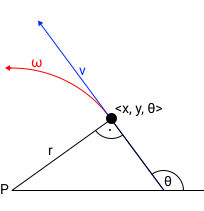
\includegraphics[width=0.5\linewidth]{img/inertial}
	\caption{
		In this diagram a slight turning motion of the robot is described by the translational velocity $v$ and angular velocity $\omega$. These velocities, if remaining unchanged, render the robot to move in a perfect circle with the center point $P$ and radius $r = | \frac{v}{\omega}|$. Even if the angular velocity remains 0 the motion is still described as a circle with an infinite radius. \footcite[Pages 95 - 107]{thrun2002probabilisticRobotics}
	}
	\label{fig:inertial}
\end{figure}



\section{Depth Sensing}
Similar to motion models contributing to robot localization in Autumn, Depth Sensing is utilized to perceive and map the drones environment. 
The technologies in this section focus on mapping distance information to each point in the cameras field of view thus providing 3D-Imaging.

\subsection{Structured Light}
One approach uses active illumination to project a varying intensity pattern onto the perceived scene thus allowing for a camera to extract 3D-information from the distorted pattern as the surface of the scene is non-planar. \footcite{geng2011StructuredLight}

\subsection{Time-of-Flight}
Time-of-Flight (ToF) sensors perform active triangulation, which is performed by emitting modulated light to be reflected by a scene, as described in Fig. \ref{fig:activeTriangulation}. The distance to the scene is determined using the time difference between emission and detection of singular rays (more prominent with ToF Laser-Scanners like LiDAR) or the phase shift of light reflected by the whole scene. The latter allows for mapping depth information to the entire Field-of-View (FoV) of a camera. 
%It may be necessary to differentiate mapping using depth perception sensors from LiDAR technologies which pose an alternative solution. 
Although LiDAR sensors fall under the category of ToF sensors they perceive the distance to an object using pulsed lasers thus outputting
the distance to singular points in the sensors environment rather than depth information mapped to an image. \footcite{gokturk2004time} \footcite{velodyne2021LiDAR}
% LiDAR verwenden die Zeitdifferenz und berechnen mittels Trigonometrie die Distanz
As 3D-LiDAR sensors applied in many commercial mapping solution are very expensive they disqualify for use in Autumn as it focuses on performing with approximate precision using relatively inexpensive camera based equipment. 

\begin{figure}
	\centering
	\includegraphics[width=0.8\linewidth]{img/activeTriangulation}
	\caption{
		This diagram depicts a ToF depth camera emitting IR-light (red) onto a surface. The camera sensor then utilizes the phase-shift $\varphi$ between the emitted (red) and received signal (blue) to calculate the distance between the scene and sensor. \footcite{altuntas2021triangulation}
		% noch mehr schreiben
	}
	\label{fig:activeTriangulation}
\end{figure}


\subsection{Stereo Vision}
The last and most significant approach to Autumn performs passive triangulation using two cameras setup as seen in Fig. \ref{fig:passiveTriangulation}. Although this eliminates the need for any light to be emitted, however the problem of correspondence is introduced, which deals with associating the different projections to the same point in the real world\footcite{ng2019StereoCorrespondence}. There are multiple approaches to this problem which are generally divided into global and local matching methods with the latter being more computationally efficient while sacrificing quality. \footcite{do2019review}

In Autumn this approach was pursued using a Stereolabs ZED depth camera as it was superior to any competitors such as the Microsoft Kinect or Intel Realsense concerning availability and cost-effectiveness. 

\begin{figure}
	\centering
	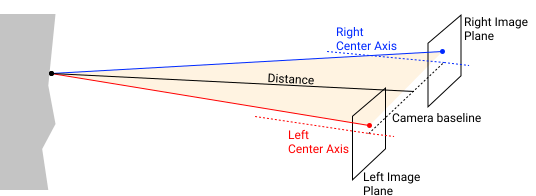
\includegraphics[width=0.8\linewidth]{img/PassiveTriangulation}
	\caption{
		This diagram describes the camera setup found in passive triangulation systems. Using stereo-photogrammetry the distance to the perceived scene is calculated.\footcite{altuntas2021triangulation}
	}
	\label{fig:passiveTriangulation}
\end{figure}

\subsection{ZED 1 vs ZED 2i}
%As mentioned in Chapter \ref{chapter:architecture} the Stereolabs ZED 1 was used in a first prototype and later replaced with a 
Chapter \ref{chapter:architecture} mentions that the Stereolabs ZED 1 used in early prototypes was quickly replaced with the ZED 2i. This change was due to processing limitations and additional features provided by the newer product version.
This section aims to benchmark the two cameras from a depth-performance standpoint to review if the upgrade enhanced depth perception thus improving the system output or if no changes were necessary when only considering depth-perception.

\subsubsection{Experiment}
To answer this question the cameras measured the vertical distance enclosed by two points mounted 1 m above each other on a stationary structure with the bottom one at a height 1 m above the ground. 
The cameras was paced on a movable rig normal to the stationary structure and 1m above the ground.  The aforementioned gap was measured by the cameras at 1 m increments between 3 m and 10 m horizontal distance measured amongst each structures base. 

The usage of ARUCO tags allowed for precisely tracking the position of each point within the camera coordinate system thus ensuring the points remain fixed even though the camera rig is moved. 
% über ARUCO schreiben
% reference zu ARUCO 
ARUCO tags are squared-based markers popular in many robotic and augmented reality applications as they provide a fast and robust solution for estimating a cameras pose relative to one or multiple markers. Each marker has a unique, identifiable pattern which allows for precisely determining and tracking its position.\footcite{jurado2015} 

\subsubsection{Results - ZED1}

Fig. \ref{plot:zed1Benchmark} depicts the mean, minimal and maximal depth-perception error measured thus indicating how well the camera performed.
To illustrate the underlying model of this data, a cubic regression is superimposed. This well fitted model indicates a relatively steady error just under 0.1 m which increases drastically after a local minima at a distance of 5.6 m. 
While the mean error increases, the minimal deviation declines to 0 m between distances of 6 m to 8 m, which would indicate a optimal interval for measurements. Although the maximal error thrives within this range it generally remains close to the mean at all other distances.
Tab. \ref{tab:resultsZed1} shows the data these findings are based on as well as a total mean, minimal and maximal deviation over all distances. 
In total the ZED 1 has a mean error of 13\% which is drastically above what the cameras data sheet states\footcite{zed1Datasheet}.

%
%The mean depth-perception error dependant on the camera distance for the ZED 1 (blue) is plotted in Fig. \ref{plot:zedBenchmark}. To illustrate the positive tendency a linear regression (cyan) is superimposed. The trend line indicates a relatively steep slope with the mean error adding up by 0.03 m at increasing distances from the rig. Additionally the error range listed in Tab. \ref{tab:errorMinimaMaxima} shows a base error of 0.7\% and a maximum mean error of 3\%, which is similar to the error stated by the cameras data sheet\footcite{zed1Datasheet}.
%
%The data for the ZED 2 (red) and its corresponding trend line (orange) indicate a much more shallow slope with 0.01 m per meter distance to the rig. Looking at the error range the ZED 2 lies below 1\% mean error at all distances which also corresponds to the data sheets specifications \footcite{zed2Datasheet}.


%When comparing each trend line for each camera it is apparent that the slope of the ZED 1 with $0.03m/m$ is more than twice as large compared to the ZED 2 at $0.01m/m$. This indicates that with increasing distance the depth-perception error increases dramatically. 
%Another interesting finding are the minima and maxima of the mean depth-perception error found in Tab. \ref{tab:errorMinimaMaxima}.
%As illustrated the ZED 1 inherits a substantially large minimal and maximal error of  $0.07m$ and $0.31m$.
%Compared to this the ZED 2 performed much better with a almost non existent base error and a maximal error of $0.1m$.

%\begin{table}[h]
%	\centering
%	\begin{tabular}{|l|l|l|}
%		\hline
%		& \textbf{Minimal Mean Error} & \textbf{Maximal Mean Error} \\ \hline
%		\textbf{ZED 1}  & 0.07 m 					  & 0.31 m                      \\ \hline
%		\textbf{ZED 2} & 0.01 m                      & 0.10 m                      \\ \hline
%	\end{tabular}
%	\caption{Table containing the minimal and maximal mean error of both the ZED 1 and ZED 2.}
%	\label{tab:errorMinimaMaxima}
%\end{table}

\begin{table}[h]
	\centering
	\begin{tabular}{|l|l|l|l|l|l|l|l|l|l|}
		\hline
		\textbf{Distances {[}m{]}}      & 3    & 4    & 5    & 6    & 7    & 8    & 9    & 10   & {\ul Total} \\ \hline
		\textbf{Mean Deviation {[}m{]}} & 0.07 & 0.08 & 0.09 & 0.08 & 0.09 & 0.14 & 0.17 & 0.31 & {\ul 0.13}  \\ \hline
		\textbf{Min Deviation {[}m{]}}  & 0.07 & 0.04 & 0.04 & 0.00 & 0.00 & 0.00 & 0.01 & 0.01 & {\ul 0.00}  \\ \hline
		\textbf{Max Deviation {[}m{]}}  & 0.08 & 0.11 & 0.13 & 0.45 & 0.67 & 0.18 & 0.24 & 0.84 & {\ul 0.84}  \\ \hline
	\end{tabular}
	\caption{Summarized data of mean, minimal and maximal deviation for the ZED 1 camera at increasing distances.}
	\label{tab:resultsZed1}
\end{table}

\begin{figure}[h]
	\begin{center}
		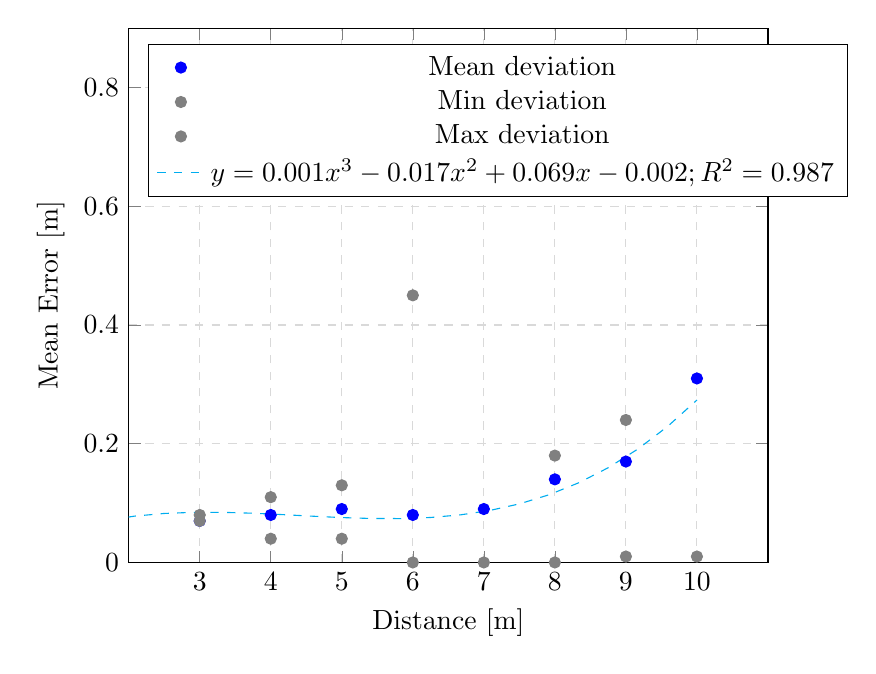
\begin{tikzpicture}
			\begin{axis}[
				width=0.8\linewidth, % Scale the plot to \linewidth
				grid=major, 
				grid style={dashed,gray!30},
				xlabel={Distance [m]}, % Set the labels
				ylabel={Mean Error [m]},
				legend pos=north west,
				xtick={3, 4, 5, 6, 7, 8, 9, 10},
				xmin=2,
				xmax=11,
				ymin=0,
				ymax=0.9,
				]
				
				
				%zed1 mean
				\addplot[only marks, color=blue]
				table[row sep=crcr]{
					distance error \\
					0 0 \\
					3 0.07 \\
					4 0.08 \\
					5 0.09 \\
					6 0.08 \\
					7 0.09 \\
					8 0.14 \\
					9 0.17 \\
					10 0.31 \\
				}; 
				\addlegendentry{Mean deviation}
				
				%zed1 min
				\addplot[only marks, color=gray]
				table[row sep=crcr]{
					distance error \\
					0 0 \\
					3 0.07 \\
					4 0.04 \\
					5 0.04 \\
					6 0 \\
					7 0 \\
					8 0 \\
					9 0.01 \\
					10 0.01 \\
				}; 
				\addlegendentry{Min deviation}
				
				%zed1 max
				\addplot[only marks, color=gray]
				table[row sep=crcr]{
					distance error \\
					0 0 \\
					3 0.08 \\
					4 0.11 \\
					5 0.13 \\
					6 0.45 \\
					7 0.67 \\
					8 0.18 \\
					9 0.24 \\
					10 0.84 \\
				}; 
				\addlegendentry{Max deviation}
				
				%zed1 mean regression
%				\addplot[no marks, color=orange, style=dashed]
%				table[row sep=crcr, y={create col/cubic regression={y=error}}]{
%					distance error \\
%					0 0 \\
%					3 0.07 \\
%					4 0.08 \\
%					5 0.09 \\
%					6 0.08 \\
%					7 0.09 \\
%					8 0.14 \\
%					9 0.17 \\
%					10 0.31 \\
%				};
				\addplot[no marks, color=cyan, style=dashed, domain=0:10] (x, 0.0013*x*x*x - 0.0171*x*x + 0.0686*x - 0.0024);
				\addlegendentry{$y = 0.001x^3 - 0.017x^2 + 0.069x - 0.002; R^2 =  0.987$} 
				
			\end{axis}
		\end{tikzpicture}
		\caption{This plot describes how the mean depth-performance error of both the ZED 1 (blue) and ZED 2 (red) Stereo Camera changes with increasing distance to an object. Furthermore the linear regression function for both the ZED 1 (cyan) and ZED 2 (orange) are plotted. 
		 }
	 	\label{plot:zed1Benchmark}
	\end{center}
\end{figure}



\subsubsection{Results - ZED 2i}

Data for the mean, minimal and maximal depth-perception error of the ZED 2i is plotted in Fig. \ref{plot:zed2Benchmark}.
%The cubic regression model for this camera indicates a coherently low mean error which decreases after a local maxima at a distance of 8.6 m. 
The cubic regression model for this camera indicates a slight negative trend with a coherently low mean error, peaking at a local maxima at 8.6 m. However the initial believe suggests that with increasing distances the error thrives correspondingly. According to the coefficient of determination $R^{2}$, indicating that the cubic regression function does not fully match the data, a different regression model may result in more accurate assertions supporting the initial believe. 
Considering the overall error range, the minimal error remains below 0.02 m for all distances while the maximal error grows to approximately 0.4 m. 
A optimal measurement zone due to moderate mean and non-existent minimal deviation can be observed between a distance of 7 m and 8 m. 
Tab \ref{tab:resultsZed2} indicates a overall mean error of 5\% which does correspond to the statement of the ZED 2i data sheet\footcite{zed2Datasheet}.



\begin{table}[h]
	\centering
	\begin{tabular}{|l|l|l|l|l|l|l|l|l|l|}
		\hline
		\textbf{Distances {[}m{]}}      & 3    & 4    & 5    & 6    & 7    & 8    & 9    & 10   & {\ul Total} \\ \hline
		\textbf{Mean Deviation {[}m{]}} & 0.01 & 0.01 & 0.06 & 0.08 & 0.05 & 0.04 & 0.10 & 0.08 & {\ul 0.05}  \\ \hline
		\textbf{Min Deviation {[}m{]}}  & 0.00 & 0.00 & 0.01 & 0.02 & 0.00 & 0.00 & 0.02 & 0.02 & {\ul 0.00}  \\ \hline
		\textbf{Max Deviation {[}m{]}}  & 0.03 & 0.11 & 0.26 & 0.24 & 0.42 & 0.35 & 0.43 & 0.41 & {\ul 0.43}  \\ \hline
	\end{tabular}
	\caption{The mean, minimal and maximal depth-perception deviation measured by the ZED 2i}
	\label{tab:resultsZed2}
\end{table}

\begin{figure}[h]
	\begin{center}
		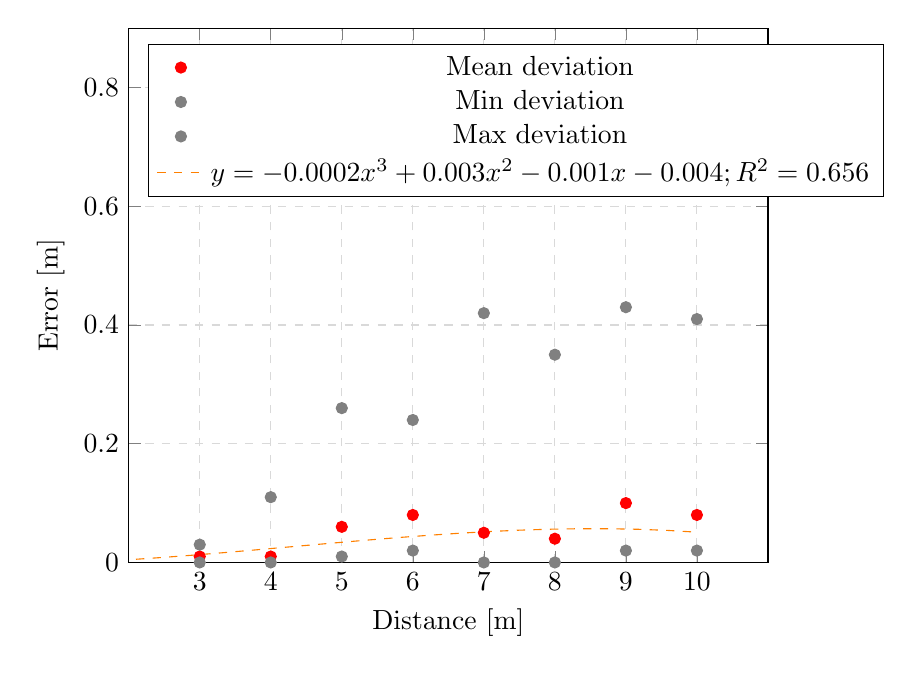
\begin{tikzpicture}
			\begin{axis}[
				width=0.8\linewidth, % Scale the plot to \linewidth
				grid=major, 
				grid style={dashed,gray!30},
				xlabel={Distance [m]}, % Set the labels
				ylabel={Error [m]},
				legend pos=north west,
				xtick={3, 4, 5, 6, 7, 8, 9, 10},
				xmin=2,
				xmax=11,
				ymin=0,
				ymax=0.9,
				]
				
				
				%zed2 mean
				\addplot[only marks, color=red]
				table[row sep=crcr]{
					distance error \\
					0 0 \\
					3 0.01 \\
					4 0.01 \\
					5 0.06 \\
					6 0.08 \\
					7 0.05 \\
					8 0.04 \\
					9 0.10 \\
					10 0.08 \\
				}; 
				\addlegendentry{Mean deviation}
				
				%zed2 min
				\addplot[only marks, color=gray]
				table[row sep=crcr]{
					distance error \\
					0 0 \\
					3 0. \\
					4 0 \\
					5 0.01 \\
					6 0.02 \\
					7 0 \\
					8 0 \\
					9 0.02 \\
					10 0.02 \\
				}; 
				\addlegendentry{Min deviation}
				
				%zed2 max
				\addplot[only marks, color=gray]
				table[row sep=crcr]{
					distance error \\
					0 0 \\
					3 0.03 \\
					4 0.11 \\
					5 0.26 \\
					6 0.24 \\
					7 0.42 \\
					8 0.35 \\
					9 0.43 \\
					10 0.41 \\
				}; 
				\addlegendentry{Max deviation}
				
				%zed2 mean regression
%				\addplot[no marks, color=cyan, style=dashed]
%				table[row sep=crcr, y={create col/cubic regression={y=error}}]{
%					distance error \\
%					0 0 \\
%					3 0.01 \\
%					4 0.01 \\
%					5 0.06 \\
%					6 0.08 \\
%					7 0.05 \\
%					8 0.04 \\
%					9 0.10 \\
%					10 0.08 \\
%				};
				\addplot[no marks, color=orange, style=dashed, domain=0:10] (x, -0.0002*x*x*x + 0.0026*x*x - 0.0006*x - 0.003);
				\addlegendentry{$y = -0.0002x^3 + 0.003x^2 - 0.001x - 0.004; R^2 =  0.656$} 
				
			\end{axis}
		\end{tikzpicture}
		\caption{
			This plot describes how increasing distances to a stationary object affect the mean (red), as well as minimal and maximal (grey) depth-performance error of the ZED 2. The model describing this data is approximated using a cubic regression (orange).
		}
		\label{plot:zed2Benchmark}
	\end{center}
\end{figure}



\subsubsection{Comparison}

Comparing both models the ZED 1 clearly shows a much more aggressive upwards trend than the ZED 2i which has a relatively monotonic mean error. 

However both cameras share a commonly low minimal error indicating that both are able to correctly and precisely take depth measurements within the tested distances. 
Although the ZED 2i generally outperforms its predecessor concerning mean deviation its maximal depth-perception error strays drastically further from the mean when compared to the ZED 1. 


%Comparing both trend lines and mean error range the ZED 1 clearly shows a much more aggressive upwards trend and higher base error compared to the ZED 2. However as the coefficient of determination $R^{2}$ for each trend line indicate a mediocre fit the aforementioned assumptions should not be solely taken into consideration when comparing the two camera systems. 

Having said this, in combination with the data sheets, the overall trend on depth-performance meets the initial assumption and justifies the upgrade to the ZED 2i.

%Considering all of the aforementioned findings it is apparent that the ZED 2 produced much better depth-perception results compared to the ZED 1. This justifies the upgrade not only from a feature focused standpoint but also quality wise as this greatly effects the final 3D point cloud utilized by components discussed later in this thesis. 

\filbreak
	\chapter{Simultaneous Localization and Mapping}
\label{chapter:slam}

\textbf{Author: Lukas Leskovar} 

%frame of reference klingt nicht so gut
The problem of localizing as well as navigating a system through a completely or partly unknown environment without any external coordinate system (i.e. GPS, Optical Beacon Tracking, etc.) has proven itself to be one of the most complex and yet fundamental topics in many scientific research fields with robotics being most prominent. The main approach to this problem is Simultaneous Localization and Mapping (SLAM) which dates back to the mid 1980s. Back then the first solutions based on Extended Kalman Filters or Rao-Blackwellised Filters were formulated. \footcite{durrantSlam2006}  \footcite{cadenaSlamFuture2016}

To date the topic of SLAM has matured, algorithms have gotten more reliable and robust and are utilized in many industries. Applications for SLAM range from Navigating a Mars Rover over autonomous cars or warehouse robots to simple household appliances like vacuum cleaners. 

As one major topic of this thesis is robot navigation in a GPS-denied area as well as mapping of such environment, different modern SLAM approaches and solutions utilized by the project team are discussed in this chapter.

\section{Localization}
%state estimation beschreiben dass pose sowie andere informationen wie geschw. usw. erfasst werden. 
Localization or state-Estimation aims to reconstruct the state of a system using interoceptive measurements (e.g. acceleration, velocity, etc.) as well as an exteroceptive model (e.g. position and orientation) of the system. \footcite{barfootStateEstimation2017}
Put into the context of mobile robotics this means that in order to perform comprehensive localization of a mobile robot a sensor fusion between on-board sensors and an external coordinate system or map ought to be performed as solely relying on incremental sensors for odometry would quickly result in large accumulated errors.
%Exemplary for such a robot would be a drone utilizing a Inertial Measurement Units (IMU) odometry as well as GPS positional data to estimate its current position.
Exemplary for such a system would be an industrial robot utilizing a construction plan to correct errors by wheel-encoded odometry as well as to navigate through a factory. 

\section{Mapping}
Contrary to localization and state-estimation, the current pose of the system is known while its environment remains uncharted.
Therefore stand-alone mapping aims to generate a model of its environment by evaluating sensor readings of environmental features as well as the systems pose to reconstruct aforementioned features in a global reference frame. 
Mapping applications often combine technologies typically found in scientific fields such as photogrammetry, computer vision or robotics. 
Another example would be a drone computing camera images and GPS positional data with a photogrammetric algorithm to reconstruct a 3D-Model of a building. 


\section{Localization and Mapping}
The aforementioned technologies are considered rather simplistic problems as either the environments map is given or reliable pose-estimation can be provided. While most applications meet either of these criteria with pre-built maps or GPS being available, in some environments such as indoors, mineshafts or outer space both the systems pose and environment remain uncertain and need to be determined simultaneously hence simultaneous localization and mapping. 
To summarize, the crux of the SLAM problem is that localizations requires a map and mapping depends on pose estimates however neither are certain. 

To approach this problem in a structured way a SLAM system usually comprises two main components:
\begin{itemize}
	\item A front-end in charge of abstracting sensory input to be used in the back-end by performing feature extraction as well as data association. 
	%Furthermore it is responsible for associating corresponding features over multiple measurements, which is typically referred to as short-term data association. Long-term data association or loop closure therefore aims to link current measurements to previously observed features thus  correcting accumulated odometry errors as well as adapting the global topology. 
	\item A back-end performing probabilistic estimation based on the abstracted data fed in by the front-end. The back-end also provides information to the front-end supporting loop closure detection. 
\end{itemize}

The following sections will mainly focus on the SLAM back-end and dissect the problem by reviewing different probabilistic approaches. 


%In order to partially solve this dilemma SLAM incorporates loop closure to correct the global map as well as positional estimates provided by odometry. A loop closure event occurs when revisiting previously mapped landmarks and associating relations between features to adapt the global topology. %Without loop closure a mobile robot would perceive its environment as a infinite corridor.


\section{Data Association}
While many aspects of the front-end remain application specific each SLAM system typically contains modules for data association in the following ways.
Short-term data association or feature tracking is responsible for associating corresponding features over multiple measurements while long-term data association aims to detect and link similarities between current measurements and previously observed features. These loops help correcting accumulated odometry errors as well as optimizing the global topology. 
A loop closure typically event occurs when revisiting previously mapped landmarks.

\section{Map Representation}
The way a robot perceives its environment and maintains a accurate map of its environment is directly dependant on many criteria such as complexity of tasks, size of its environment as well as measurement quality mainly influenced by sensor noise. 
Tailoring to benefit some of the aforementioned criteria most robotic mapping systems utilize either of two paradigms, metric or topological, each proposing their respective strengths and weaknesses.

Metric or grid-based maps build a map of the robots environment as occupancy grids, with each grid cell indicating the presence of an obstacle. The main benefit using metric maps is the facilitated construction of large-scale mappings as well as non-ambiguous determination of places. However such maps have significant drawbacks concerning space as well as time complexity and require accurate pose estimation of the robot.

Topological or feature-based maps reconstruct their environment as graphs with each node representing a feature or landmark perceived by the robots sensors. In contrast to metric maps they allow for comprehensive path planning and are significantly more compact as its resolution is directly proportional to the environments complexity. \footcite{thrunMaps1998}

 





\section{Problem Definition}


\section{Solution Paradigms} 

\subsection{Kalman Filter}

\subsection{Particle Filter}

\subsection{Graph-based}


\section{Visual SLAM}


%\section{Application Scenarios}
%
%\subsection{Map Acquisition}
%
%\subsection{Black-Box Localization}
%
%\subsection{Continuos Map Exploration}
%
%
%\section{2D SLAM}
%
%\subsection{Evidence Grid-based SLAM}
%
%\subsection{Graph-based SLAM}
%
%\subsection{Feature-based SLAM}
%
%
%\section{3D SLAM}
%
%\subsection{Visual SLAM}
%
%\subsection{Graph-based SLAM}
%
%
%\section{Obtaining Odometry}
%
%\subsection{Wheel Encoder Odometry}
%
%\subsection{Visual Odometry}
%
%\subsection{Visual Inertial Odometry}


\section{Loop Closure for Visual SLAM}

\subsection{Appearance-based}

\subsection{Deep Learning}


\section{Map optimization}

\subsection{Bundle Adjustment}



\filbreak
	
	\chapter{Representation of Environments}

\textbf{Author: Fabian Kleinrad} 

\section{Abstract Environments}

\subsection{Abstraction Levels}

\section{Abstraction Methods in Autumn}

\subsection{Occupancy Grid}

\subsection{Point Cloud}

\subsection{ROS Types}

\section{Abstracted Environments in Autumn}

\subsection{autumn$\_$pathfinding$\_$2D}

\subsection{autumn$\_$pathfinding}
	
	\chapter{Path Planning}

\textbf{Author: Fabian Kleinrad} 

A crucial part of autonomy in robotics are means for planning ahead movements in a cooperative manner with the environment. Means to accomplish this are so called path planning algorithms. This chapter is going to focus on exploring the different kind of approaches to path planning and evaluate which approach is most fitting to be used in a real-time, high-dimensional use case present in the Autumn project.


\section{Algorithm Variants}

The problem of finding an optimal path between two points is an old one.
The first proposed solution was the Dijkstra's Algorithm. However with steadily evolving computer science the challenges to be master by such Algorithms got harder and harder. That's the reason why over the last years the simple principle of the Dijkstra Algorithm has branched out specializing and excelling in certain real world applications.
\footcite{Pan2020}

\subsection{Sampling-based Algoritms}

\subsection{Multiple Query}

\subsection{Single Query}

\section{PRM}

\subsection{Core Principles}

\subsection{How it works}

\section{RRT Algorithm}

\subsection{Core Principles}

\subsection{How it works}

\section{A* Algorithm}

\subsection{Core Principles}

\subsection{How it works}

\section{Comparison RRT with A*}

\subsection{Purpose of RRT}

\subsection{Purpose of A*}

\subsection{Better choice for UAV application}

\section{RRT* Algorithm}

\subsection{Difference to RRT}

\subsection{How it works}

\section{Other RRT Variants}

\subsection{RT-RRT}

\subsection{Smart-RRT}

	\chapter{Collision Detection}
\label{chapter:collision_detection}

\textbf{Author: Fabian Kleinrad} 

This chapter will concern itself with the method of detecting collisions within the path planning phase. The needed information about the environment stems from the data structures covered in Chapter \ref{chapter:abstract_env}. 

\section{Fundamental Principle}
An essential part of autonomy in robotics is the aspect of collision avoidance. This is only possible if the robot has the means to identify and detect possible collisions and act suitably to circumvent collisions from happening.\newline
In Autumn, this step of collision detection happens alongside path planning. With collision detection being a very cost-intensive process, it is essential to optimize the algorithm for better performance while simultaneously keeping a safety margin. This safety margin is especially important since the algorithm controls a UAV. 

\subsection{Base Algorithm}
The principle of collision detection is elementary due to the organized and semi-organized data structures the algorithm uses. A function can be called that checks for collisions. It takes Cartesian coordinates as parameters and returns a value that indicates if an obstacle is present or not. All the collision detection algorithm has to do is check if there are any collisions between two points sampled by the path planning algorithm. To accomplish this task, Bresenham's Algorithm will be used.\newline

\subsubsection{Bresenham's Algorithm} 
Bresenham's Algorithm is a solution to the problem of rasterizing curves, rasterizing being the process of converting curves or lines into cells on a grid, representing the same shape. The Algorithm covers many different shapes, but only a straight line will be necessary because of the nature of the path planning algorithm.
The algorithm works by calculating an error for each candidate cell. The formula for this error being: $e=(y-y_0)dx-(x-x_0)dy$. Hereby $x$ and $y$ are the coordinates of the cell the error is calculated for, which are being subtracted by the coordinates of the starting point. $dx$ and $dy$ are the differences between the first and last point of the line.
The error symbolizes the deviation from the original line. Calculating the errors for each cell makes it possible to choose cells best representing the original line.\footcite{Zingl2012}

\begin{algorithm}[]
	\caption{Bresenham's Line Algorithm\footcite{Zingl2012}}
	\SetKwFunction{Fabs}{abs}
	\SetKwFunction{FUsePixel}{UsePixel}
	$dx \gets \Fabs(x_1-x_0)$\;
	$dy \gets \Fabs(y_1-y_0)$\;
	$sx \gets x_0<x_1 ? 1 : -1$\;
	$sy \gets y_0<y_1 ? 1 : -1$\;
	$error \gets dx + dy$\;
	\While{$x_0 \neq x_1$ and $y_0 \neq y_1$}{
		$\FUsePixel(x_0, y_0)$\;
		$e_2 \gets error * 2$\;
		\If{$e_2 \geq dy$}{
			$error \gets error + dy$\;
			$x_0 \gets x_0 + sx$\;
		}\If{$e_2 \leq dx$}{
			$error \gets error + dx$\;
			$y_0 \gets y_0 + sy$\;
		}
	}
\end{algorithm}

%\begin{figure}[h]
%	\centering
%	\includegraphics[width=0.5\linewidth]{img/Bresenhams}
%	\caption{Application of Bresenham's Algorithm to a straight line, %with visible errors. \cite{Zingl2012}}
%	\label{fig:collision_detection_bresenham}
%\end{figure}


\section{Implementation}
The collision detection logic is in effect every time a new point is added to the graph. The path planning algorithm samples a random point and calculates its nearest neighbour. After that, a function is called, which takes two points and checks for collision on a straight-line path between these two points.\newline
A problem that arises when using it this way is the not accounted for dimensions of the drone. For that, the function takes a third parameter defining the search radius. Using this method, paths can be generated suitable for the physical drone. However, this is accompanied by an increase in computational time, which stems from how this radius, $r$, is used. For every cell that is not the first and last cell, $2r$ neighbouring cells in a line opposite the line's direction get checked. For the first and last cell, the radius translates to the circle where cells get checked. In order to not overlap validation areas, on the first and last cell, only a semicircle is being covered. 

\begin{figure}[h]
	\centering
	\includegraphics[width=0.8\linewidth]{img/CheckedPixels}
	\caption{Visualization of checked pixel in paths. Green being start/end points, red the lines calculated by the Bresenham's Algorithm and yellow the additionally checked cells with $r = 2$ .}
	\label{fig:collision_detection_checkedPixels}
\end{figure}

Therefore the to be checked cells can be calculated in dependency of the line length $l$ and radius $r$. $l$ thereby being the number of cells present in the line calculated by Bresenham's Algorithm. 
\[C=r^2+(l-2)*2r\]

\subsection{3 dimensional space}
Using this concept in a 3-dimensional environment only requires adding the new third dimension. Bresenham's Algorithm is easy to translate into the third¹2 dimension. The problem that arises is performance. When adding the radial search, it increases the total cells checked by \(C^2 - l\).  

\section{Experiment}

In order to be able to assess the practical impact of the collision detection performed by the autumn pathfinding algorithm, an experiment was conducted, which illustrates the computational time needed to guarantee no collisions from happening.

\subsection{Experimental Setup}

The experiment is split into two parts: the impact of collision detection on the computational time of two-dimensional and three-dimensional path-finding.
To get significant data, which can represent various scenarios in which the algorithm has to perform, a setup was selected to cover all aspects of the algorithm. The experiment works by planning a path through a static environment. This environment stays the same for all iterations of one algorithm and the two different variations of the algorithm. To get conclusive evidence concerning the collision detection, which is not polluted by the random nature of the algorithm, the sample size has been set to 100. \newline One sample refers thereby to a path planning with consistent parameters. The parameters are
\begin{itemize}
	\item the number of iterations of the RRT* algorithm($i$),
	\item the distance between the start and end node($d$), and
	\item the spacing of the nodes of the expanding tree($D$).
\end{itemize}
These three parameters stay constant throughout the entire duration of the experiment, the reason being that these three Parameters affect the parts of the path planning algorithm that aren't of concern in this experiment. The Parameter controlling the collision detection behaviour is the radius($r$).
For each radius, 100 paths are generated, and each execution of the algorithm is timed from the point of the function call till the return of the calculated path. 
The set of radii to be tested depends on the space in which paths are generated.
For each radius, the meantime of all 100 data points is calculated. This results in data representing how collision detection impacts the computational time of the autumn path-planning algorithm.

\subsection{Two-dimensional Algorithm}

For autumn\_pathplanning\_2d, radii starting from zero, resulting in disabling collision detection functionality, up to two 2000, with a step size of 100, have been tested. In figure \ref{plot:2dCollisionExp} the linear relationship between collision detection and the computational time can be observed. Furthermore, it can be derived from this plot that the two-dimensional path planning algorithm can handle high amounts of collision checks without making the path calculation unusable. On average, an additional 100 in radius results in a 90ms longer runtime. In this context, it should be pointed out that the radii chosen in this experiment are not in relation to radii used in practical application. For a 0.05 resolution of the occupancy grid used, radii in a range from 15 to 50 are practical. Nevertheless, this accentuated representation with a correlation coefficient of nearly one can also be applied to the practical values.   

\begin{figure}[h]
	\begin{center}
		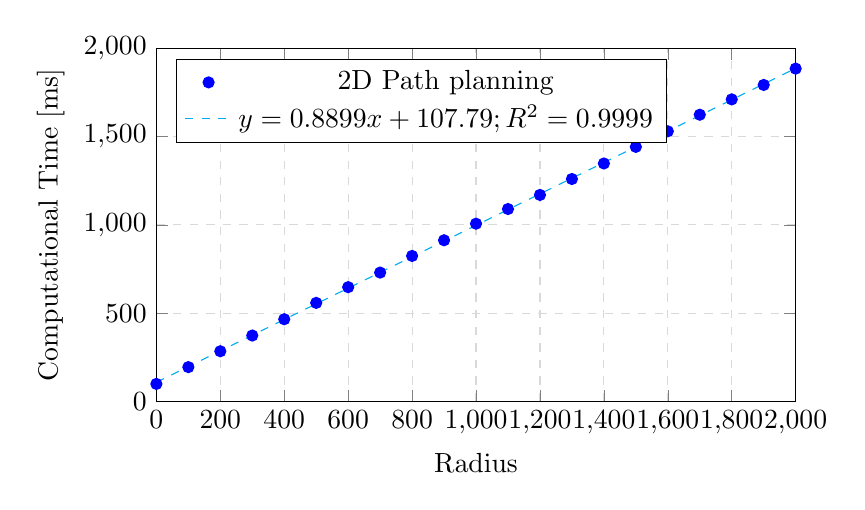
\begin{tikzpicture}
			\begin{axis}[
				height=0.5\linewidth,
				width=0.8\linewidth, % Scale the plot to \linewidth
				grid=major, 
				grid style={dashed,gray!30},
				xlabel={Radius}, % Set the labels
				ylabel={Computational Time [ms]},
				legend pos=north west,
				xmin=0,
				xmax=2000,
				ymin=0,
				ymax=2000,
				]
				
				
				%2d test data
				\addplot[only marks, color=blue]
				table[row sep=crcr]{
					0 98.853165 \\
					100 193.98699\\
					200 283.95058\\
					300 373.10144\\
					400 465.5869\\
					500 558.11993\\
					600 647.20301\\
					700 729.78178\\
					800 824.24182\\
					900 912.9868\\
					1000 1007.04737\\
					1100 1090.12372\\
					1200 1169.9529\\
					1300 1260.2584\\
					1400 1348.2436\\
					1500 1442.4541\\
					1600 1530.6858\\
					1700 1624.6226\\
					1800 1711.6543\\
					1900 1793.4719\\
					2000 1885.9677\\
				}; 
				\addlegendentry{2D Path planning}
				
				%2d test regression
				\addplot[domain=0:2000, samples=100,no marks, color=cyan, style=dashed]
				{0.8899*x + 107.79};
				\addlegendentry{$y = 0.8899x + 107.79; R^2 =  0.9999$} 
			\end{axis}
		\end{tikzpicture}
		\caption{This plot illustrates the increase in computational time with increased collision detection, for the two-dimensional path-planning algorithm. Each point represents the average time needed to compute 100 paths, with equivalent parameters.}
		\label{plot:2dCollisionExp}
	\end{center}
\end{figure}

\subsection{Three-dimensional Algorithm}

The three-dimensional algorithm was tested with values ranging from $10$ to $320$, with an increment of $2^n * 10$. Figure \ref{plot:3dCollisionExp} illustrates the result of the experiment performed using the autumn\_pathplanning algorithm. The exponential relationship between the number of collision checks and computational time is apparent. With a block size of the point cloud of 0.01, the radii used in practice would range from 20 up to 150.

\begin{figure}[h]
	\begin{center}
		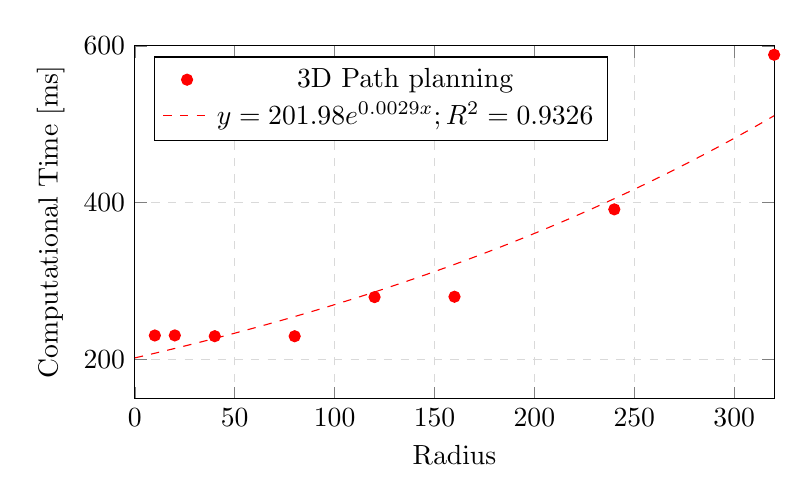
\begin{tikzpicture}
			\begin{axis}[
				height=0.5\linewidth,
				width=0.8\linewidth, % Scale the plot to \linewidth
				grid=major, 
				grid style={dashed,gray!30},
				xlabel={Radius}, % Set the labels
				ylabel={Computational Time [ms]},
				legend pos=north west,
				xmin=0,
				xmax=320,
				ymin=150,
				ymax=600,
				]
				
				
				%2d test data
				\addplot[only marks, color=red]
				table[row sep=crcr]{
					10 230.5572793  \\
					20 230.6465518  \\
					40 229.669491   \\
					80 229.5970721  \\
					120 279.5138153 \\
					160 279.9739437 \\
					240 391.4133536 \\
					320 588.5701149 \\
				}; 
				\addlegendentry{3D Path planning}
				
				%2d test regression
				\addplot[domain=0:320, samples=100,no marks, color=red, style=dashed]
				{201.98*e^(0.0029*x)};
				\addlegendentry{$y = 201.98e^{0.0029x}; R^2 =  0.9326$} 
			\end{axis}
		\end{tikzpicture}
		\caption{In this plot the correlation between increased collision detection and computational time, for the three-dimensional path-planning algorithm. }
		\label{plot:3dCollisionExp}
	\end{center}
\end{figure}

	
	\chapter{Custom Parts}

\textbf{Author: Fabian Kleinrad} 

This chapter is going to take a look at the practical side of the autumn project. When working with hardware there is the inevitable need for parts fit for the underling application. In case of autumn, with the Matrice 100 being in the center of the project the need arises to design and manufacture parts in order to make the hardware portion in autumn come together without any complication and potential weak points in the final product.

\section{Reasons}

The goal of the autumn project being as innovative and unique in terms of methods used in the realization of the project, parts needed are either not readily available or not compliant with the budget. Another difficulty are parts too specific for there to be any commercially available. Therefor to guaranty the reusability and reliability of the final product, methods to design and produce parts specifically tailored to the needs in the autumn project have to be utilized.

\subsection{Camera Mount}

Autumn conquers the problem of mapping an environment with the use of a drone. Therefore it is necessary to attach the camera used to capture the surrounding to the drone that allows it to move through that space. In case of autumn the camera being used is a ZED2i, which needs to be securely attached to an Matrice 100. Additionally to the cost factor and accompanied risk of damaging the hardware in use, the positioning and angle are important properties to consider. For that reason a commercial solution is precluded.

\subsubsection{First approach}

When working with the principle of fast prototyping, the drawback of first approaches being incomplete is inherit. Following this principle lead to attaching the ZED2i to the Matrice 100 with the help of zip ties. Rational for this decision being the reliability and strength of zip ties which allowed the camera to be secured tightly. This was important because of the need to test segments of the autumn project, worked on separately and isolated from one another. With taking simple and easy to realize steps it enables the project to progress more smoothly and without the need for other sub-areas to be set on hold because of long tedious planing and manufacturing periods of parts like an custom camera mount for a drone.

\subsubsection{Problems without a Mount}

After a period of testing with a prototype problems arise with the need of correction. In case of an, what most people consider a work-around rather than a solution to the problem of mounting a camera, they can be, in case of this application, divided in two categories.
The first aspect to consider when mounting a camera to a drone is its field of view. With UAVs hovering above ground an angle is needed in order to be able to capture details close to the ground.  

\begin{figure}[h]
	\centering
	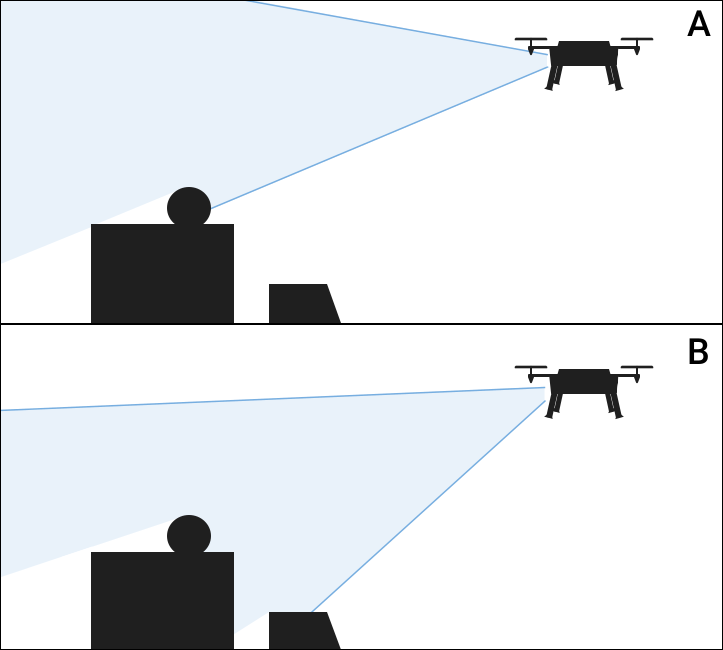
\includegraphics[width=0.7\linewidth]{img/FieldOfView}
	\caption{Depiction of the FOV for cameras mounted at different angles on a drone.\newline A: camera mounted vertically, B: camera mounted with a downward pointing angle.}
	\label{fig:custom_parts_FOV}
\end{figure}

\subsubsection{How the mount was made}

\section{CAD Software}

\subsubsection{Fusion 360}

\section{Manufacturing Process}

\subsection{Methods}

\section{3D Printing}

\subsection{FDM Printing}

\subsection{SLA Printing}
	
%	\chapter{Methodology}

\textbf{Author: } 

\filbreak

%	\chapter{Implementation}

\textbf{Author: } 

\filbreak
%	\chapter{Experiment 1}

\textbf{Author: } 

\filbreak
%	\input{sections/lessons_learned}
%	\chapter{Experiment 2}

\textbf{Author: } 


\filbreak

	\chapter{Conclusion}

\textbf{Author: Fabian Kleinrad} 

\section{Autumn Result}

The objective of the autumn project being a fully autonomous drone to be able to create 3D scans of hard to get to environments. Additionally on basis of the technologies used it is possible to deploy the drone in areas lacking a GPS signal. With these general conditions there was also an effort to keep hardware cost minimal. This leads to the final design of the autumn drone. A stereo camera was chosen due to low cost compared to technologies used for commercial autonomous solutions. The drone used in the autumn project provides for a wide range of possible sensor configuration and a high payload capacity. In the current version of the autumn drone only semi-autonomous flight is supported. Due to the lack of testing possibilities and the risk that accompanies testing autonomous drones, flight capabilities were only assessed using human input.   

\section{Mapping}
With the focus of autumn being, to be able to create 3D models of environments, mapping is a crucial part in the whole project. Mapping was realized using a SLAM algorithm, that enabled the use of a stereo camera.
SLAM generates a point cloud representing the environment the drone explores. All mapping logic is computed on the drone using a NVIDIA-Jetson, which provides enough computational power to ensure a clean model. In order to transfer the point cloud data, the jetson hosts an access point over which data is sent using ROS. This enables the user to get a real-time view of the model and how it is being constructed. The resulting point-cloud can then be used as reference material for example in a life-like render.

\section{Path-Planning}
Autonomous implies means to be able to move through an environment. In autumn this is realized via path-planning algorithm based on the model generated by the SLAM algorithm. The path is calculated separate from the drone and then sent over a wifi connection using ROS. By separating the path computation onto an external device it enables the drone to work more efficiently and the path-planning algorithm to not be constricted by computational restriction present when computing on the drone itself. The path is planned between the position of the drone and an user defined point. It gets checked each time new mapping data is available and adjusted if necessary. Depending on the mapping output path-planning can happen in two-dimensional or three-dimensional space. 

\section{Outlook}
At current times fully autonomous flight is not possible with the autumn drone. This is among other things due to the lack of sensors equipped to the drone. In the current stage the drone has no way to tell if obstacles are directly above it. This results in problems when using three dimensional path-planning because of the uncertainty of what lies above. Another problem is the short battery life-time of the drone, which is a result of the size of the drone.\newline
The modular structure provided by ROS in the autumn project allows it to be easily implemented using different hardware. For future projects it is possible to realize fully autonomous flight, using a smaller drone and a simple two-dimensional lidar. This results in the loss of three-dimensional mapping capabilities but enables more reliable and easier environment exploration. Furthermore through using ROS every part of the autumn logic can be used in separate projects where needed. An example would be using the two-dimensional path-planning algorithm in order to plan ahead the movement of an ground vehicle. 

\filbreak
	
	
	% Index
	\newpage
	\chapter*{Index}
	\printindex[name]
	\printindex[title]

	\printbibliography
	
	\chapter*{Appendix}
\label{chapter:appendix}

\includepdf[pages=-]{PROTOKOLL.pdf}

\includepdf[pages=-]{LeskovarArbeitsprotokoll.pdf}

%\includepdf[pages=-]{KleinradArbeitsprotokoll.pdf}
	
	\input{sections/messbox}
\end{document}
